\subsection{Direction Cosine Matrix}
\[
    \bm{C}_n^b = \begin{bmatrix}
        \cos\theta\cos\psi & \cos\theta\sin\psi & -\sin\theta \\
        -\cos\phi\sin\psi+\sin\phi\sin\theta\cos\psi & \cos\phi\cos\psi+\sin\phi\sin\theta\sin\psi & \sin\phi\cos\theta \\
        \sin\phi\sin\psi+\cos\phi\sin\theta\cos\psi & -\sin\phi\cos\psi+\cos\phi\sin\theta\sin\psi & \cos\phi\cos\theta
    \end{bmatrix}
\]
\[
    \bm{C}_e^n = \begin{bmatrix}
        \cos\phi & -\sin\phi\sin\lambda & \sin\phi\cos\lambda \\
        0 & \cos\lambda & \sin\lambda \\
        -\sin\phi & -\cos\phi\sin\lambda & \cos\phi\cos\lambda
    \end{bmatrix}
\]


    \begin{figure}[H]
        \centering
        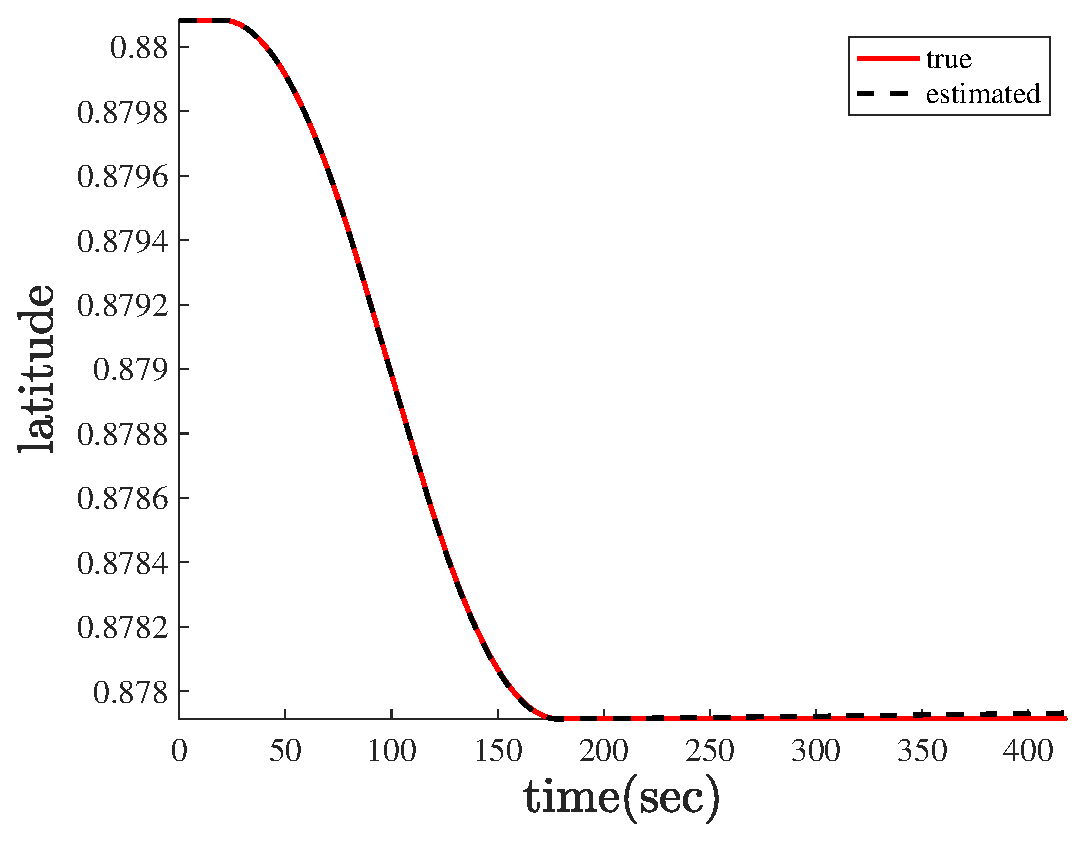
\includegraphics[width=0.7\textwidth]{../Figure/Q5/latitude_cos}
        \caption{Latitude}
    \end{figure}
    \begin{figure}[H]
        \centering
        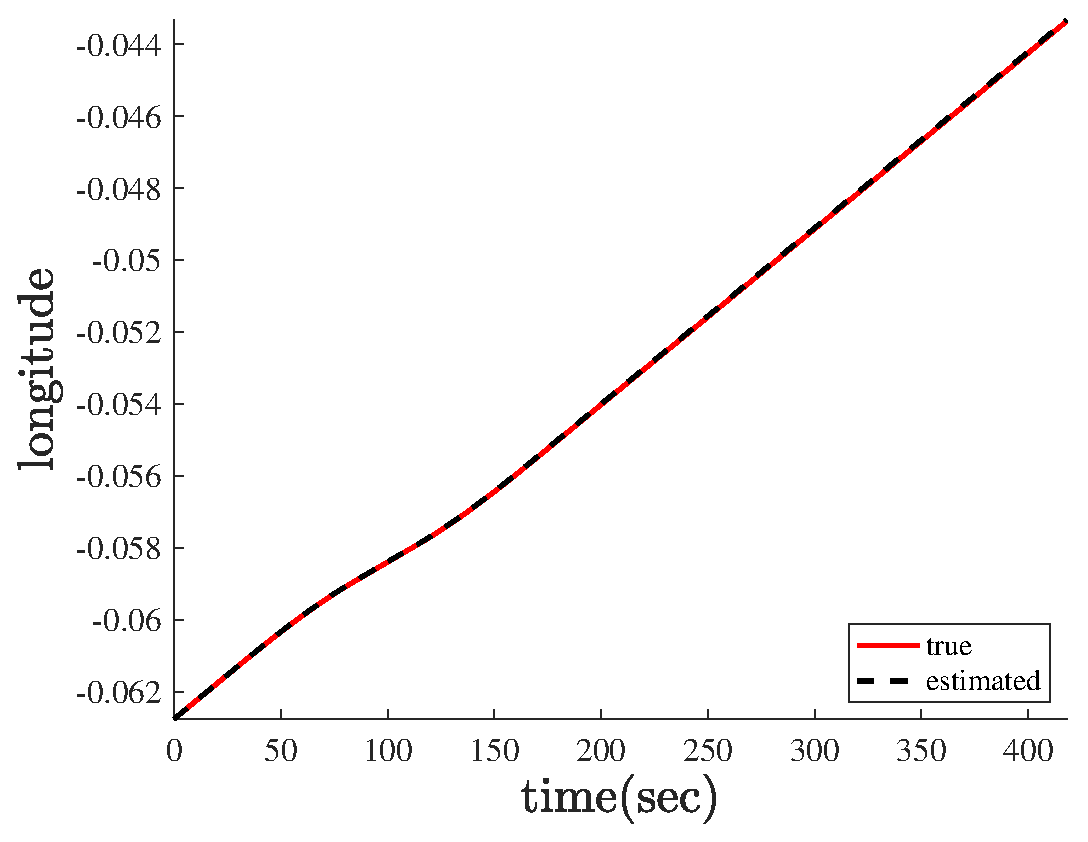
\includegraphics[width=0.7\textwidth]{../Figure/Q5/longitude_cos}
        \caption{Longitude}
    \end{figure}
    \begin{figure}[H]
        \centering
        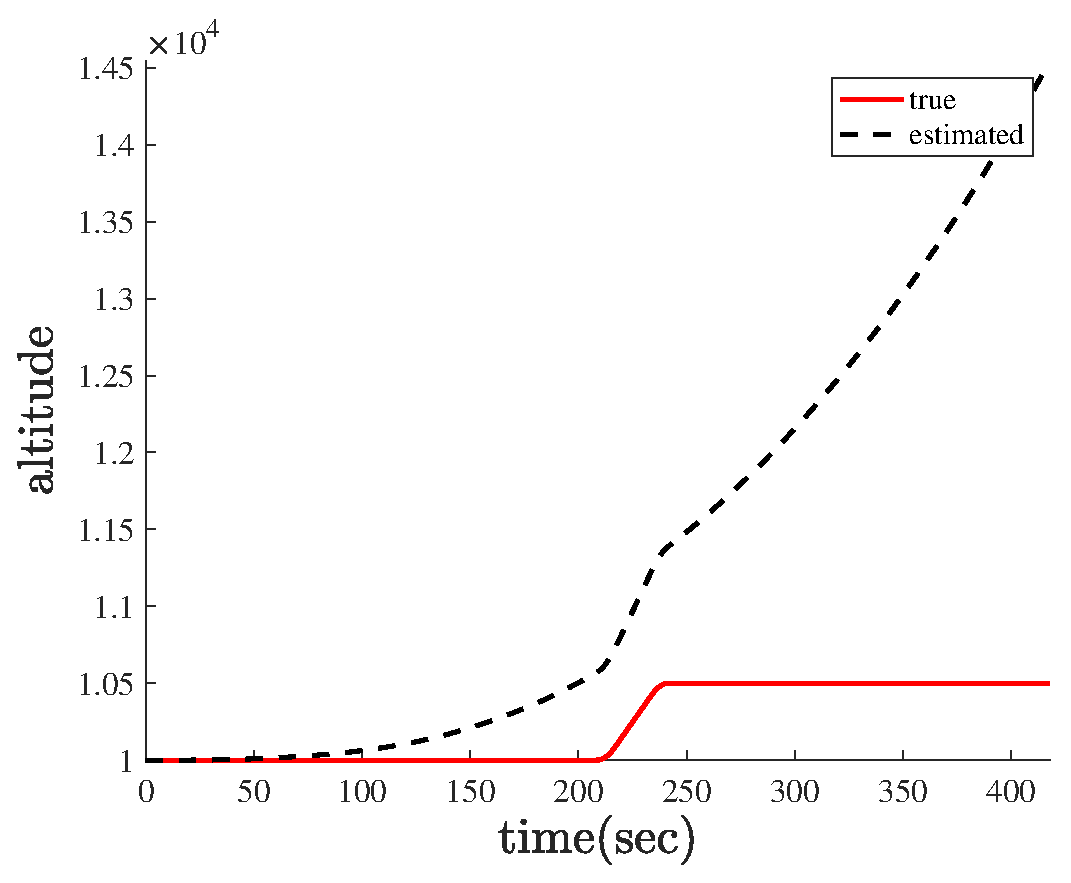
\includegraphics[width=0.7\textwidth]{../Figure/Q5/altitude_cos}
        \caption{Altitude}
    \end{figure}
    \begin{figure}[H]
        \centering
        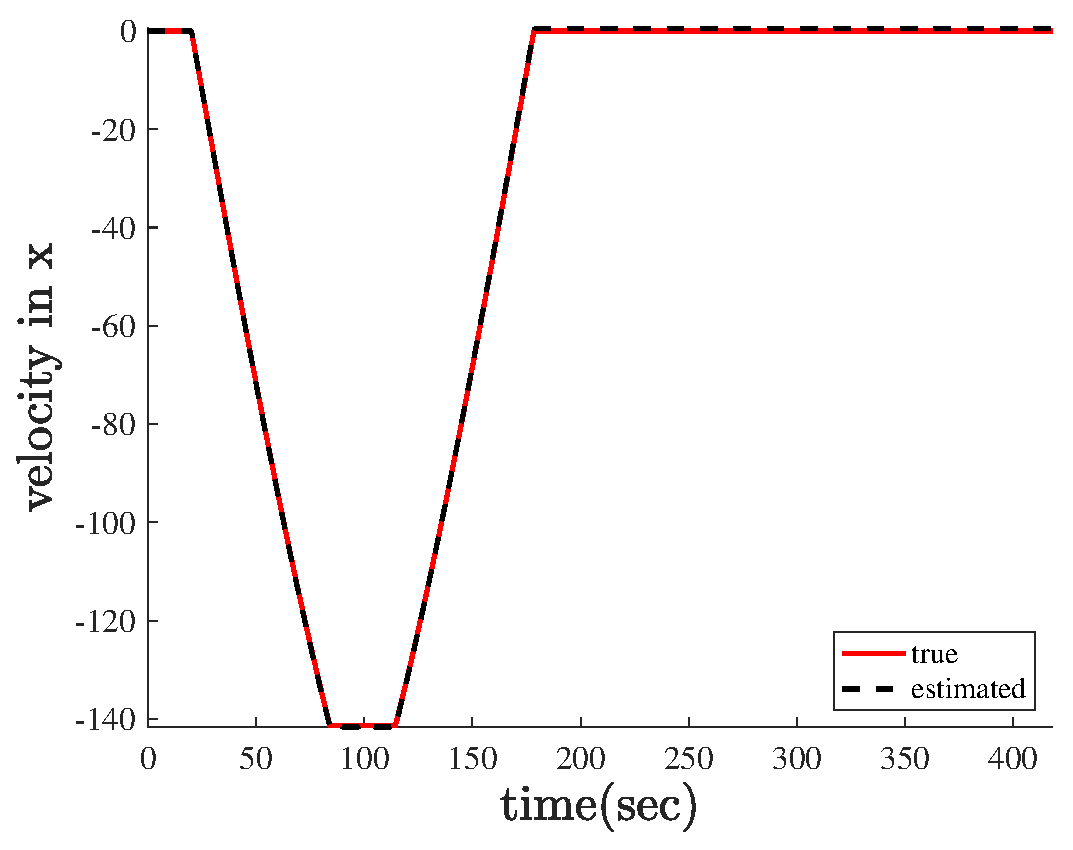
\includegraphics[width=0.7\textwidth]{../Figure/Q5/velocity_x_cos}
        \caption{Velocity in x direction}
    \end{figure}
    \begin{figure}[H]
        \centering
        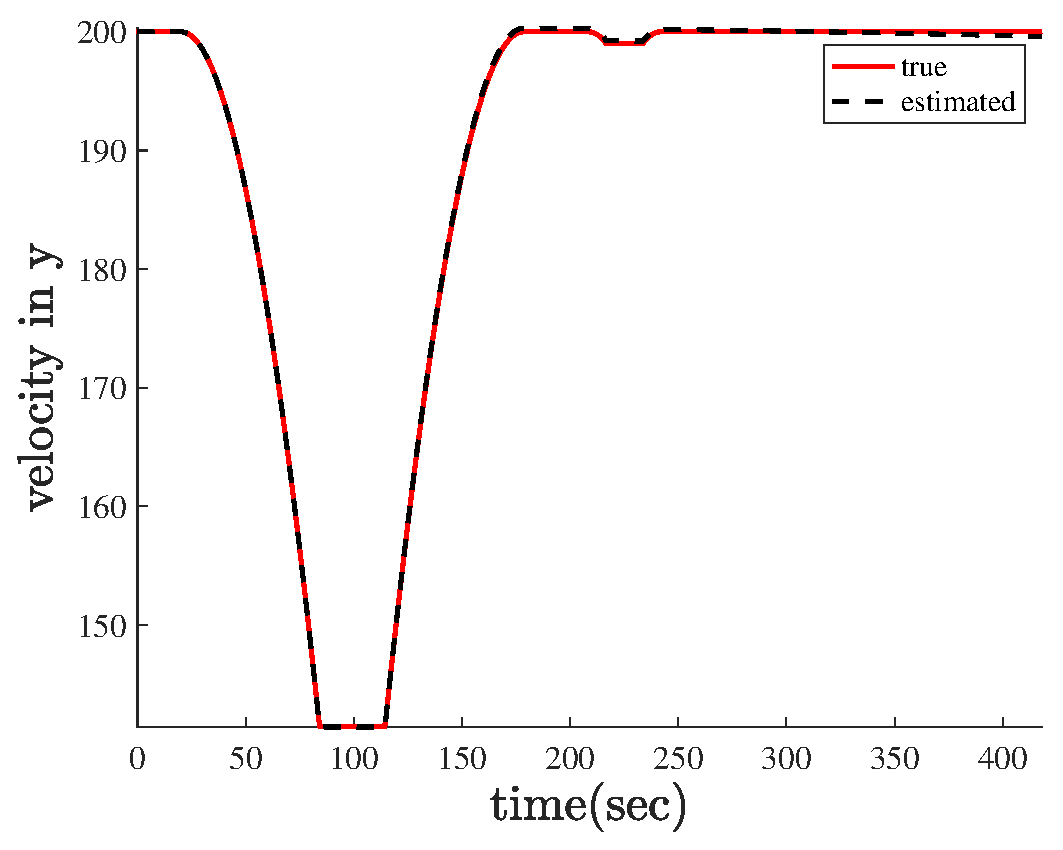
\includegraphics[width=0.7\textwidth]{../Figure/Q5/velocity_y_cos}
        \caption{Velocity in y direction}
    \end{figure}
    \begin{figure}[H]
        \centering
        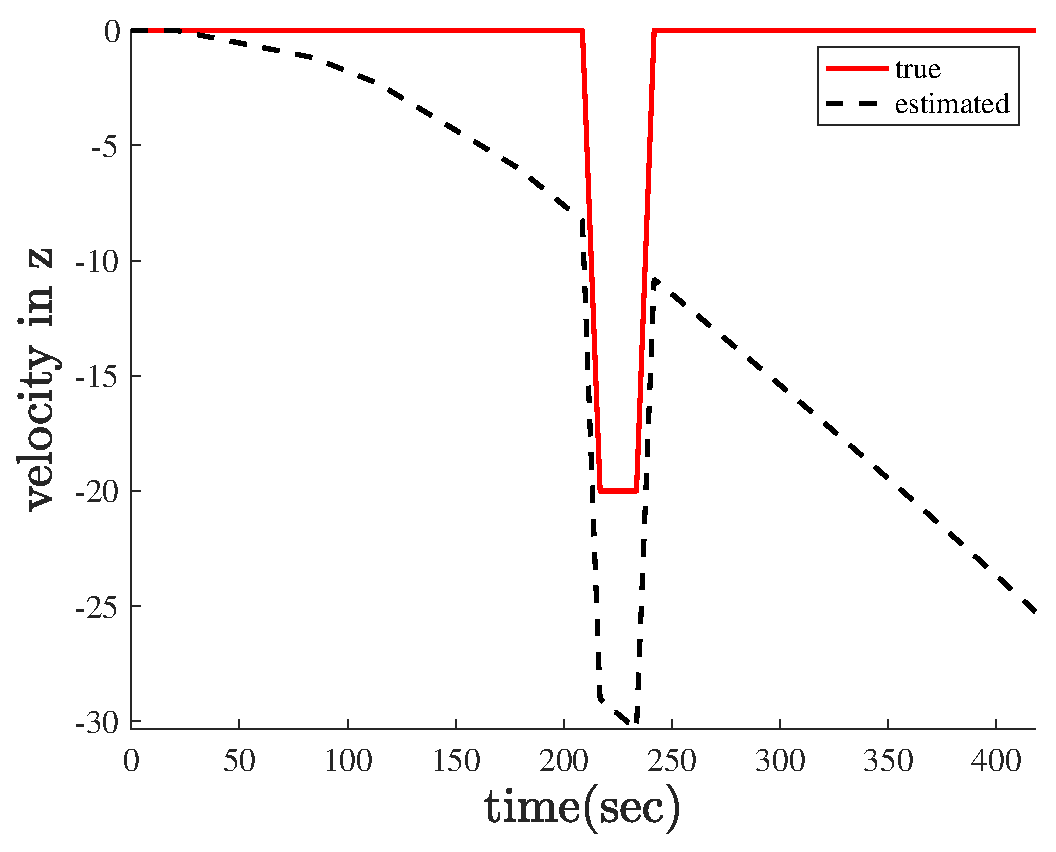
\includegraphics[width=0.7\textwidth]{../Figure/Q5/velocity_z_cos}
        \caption{Velocity in z direction}
    \end{figure}
    
    \begin{figure}
        \centering
        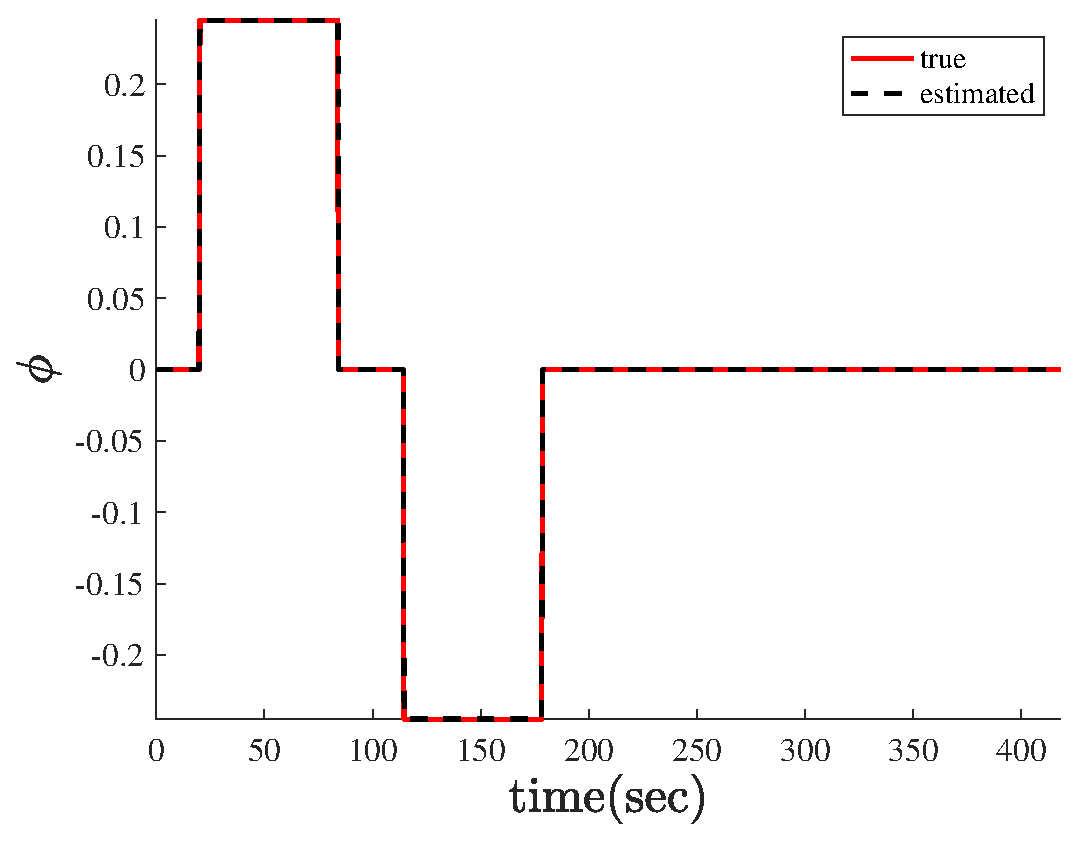
\includegraphics[width=0.7\textwidth]{../Figure/Q5/phi_cos}
        \caption{Roll}
    \end{figure}
    \begin{figure}
        \centering
        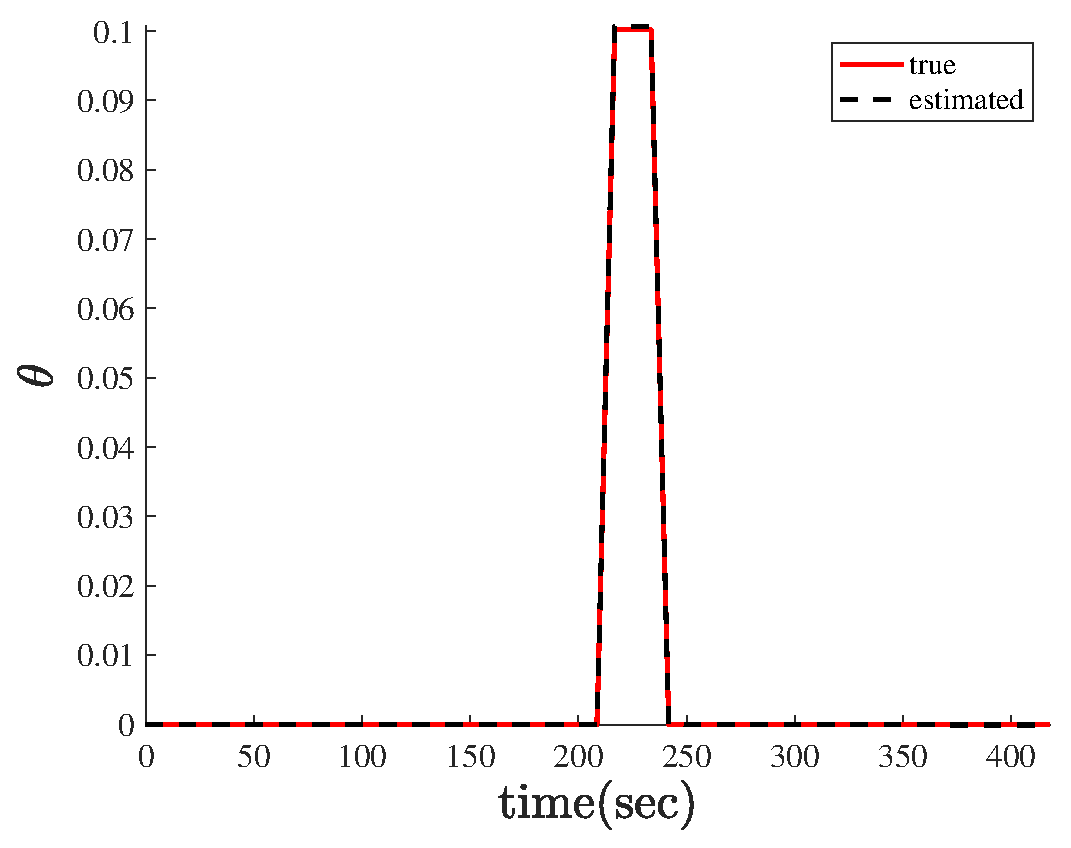
\includegraphics[width=0.7\textwidth]{../Figure/Q5/theta_cos}
        \caption{Pitch}
    \end{figure}
    \begin{figure}
        \centering
        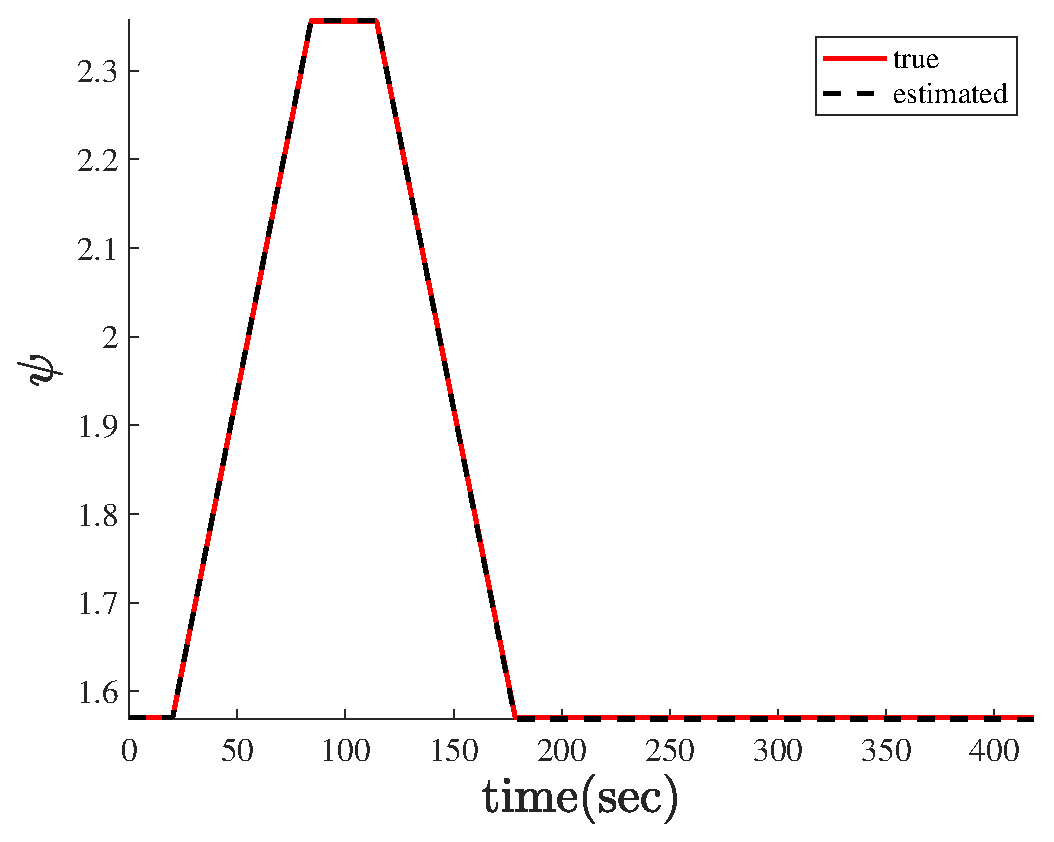
\includegraphics[width=0.7\textwidth]{../Figure/Q5/psi_cos}
        \caption{Yaw}
    \end{figure}
